
\begin{center}
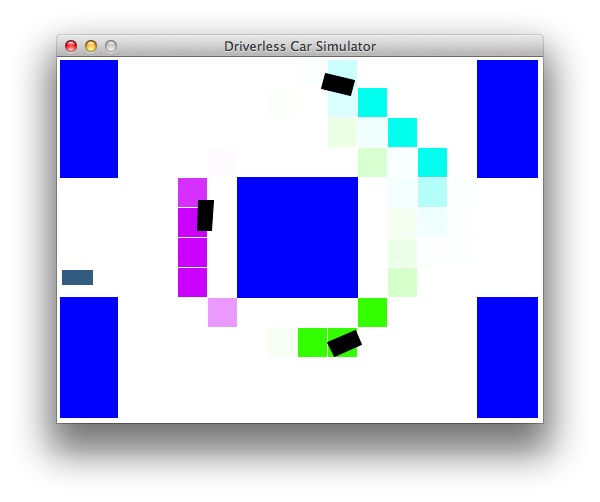
\includegraphics[width=0.5\textwidth]{media/car3.png}
\end{center}

{\bf Introduction}

This assignment is a modified version of the
\href{http://stanford.edu/~cpiech/cs221/homework/prog/driverlessCar/driverlessCar.html}
{Driverless Car} assignment written by Dr. Chris Piech.

A \href{http://en.mercopress.com/2013/03/18/in-2010-there-were-1.24-million-road-traffic-related-deaths-worldwide-says-who-report}
{study} by the World Health Organization found that road accidents kill a
shocking 1.24 million people a year worldwide. In response, there has been great
interest in developing \href{https://en.wikipedia.org/wiki/Autonomous_car}
{autonomous driving technology} that can drive with calculated precision and
reduce this death toll. Building an autonomous driving system is an incredibly
complex endeavor. In this assignment, you will focus on the sensing system,
which allows us to track other cars based on noisy sensor readings.
\clearpage

{\bf Getting started.}

You will be running two files in this assignment - |grader.py| and |drive.py|.
The |drive.py| file is not used for any grading purposes, it's just there to
visualize the code you will be writing and help you gain an appreciation for how
different approaches result in different behaviors (and to have fun!). Start by
trying to drive manually.

\begin{lstlisting}
python drive.py -l lombard -i none
\end{lstlisting}

You can steer by either using the arrow keys or `w', `a', and `d'. The up key
and `w' accelerates your car forward, the left key and `a' turns the steering
wheel to the left, and the right key and `d' turns the steering wheel to the
right. Note that you cannot reverse the car or turn in place. Quit by pressing
`q'. Your goal is to drive from the start to finish (the green box) without
getting in an accident. How well can you do on the windy Lombard street without
knowing the location of other cars?  Don't worry if you're not very good; the
teaching staff were only able to get to the finish line 4/10 times.  An accident
rate of 60\% is pretty abysmal, which is why you're going to use AI to do this. 

Flags for |python drive.py|:
\begin{itemize}
  \item |-a|: Enable autonomous driving (as opposed to manual).
  \item |-i <inference method>|: Use |none|, |exactInference|, |particleFilter|
  to (approximately) compute the belief distributions over the locations of the
  other cars.
  \item |-l <map>|: Use this map (e.g. |small| or |lombard|). Defaults to
  |small|.
  \item |-d|: Debug by showing all the cars on the map.
  \item |-p|: All other cars remain parked (so that they don't move).
\end{itemize}
\clearpage

{\bf Modeling car locations.}

Assume that the world is a two-dimensional rectangular grid on which your car
and $K$ other cars reside. At each time step $t$, your car gets a noisy estimate
of the distance to each of the cars.  As a simplifying assumption, assume
that each of the $K$ other cars moves independently and that the noise in sensor
readings for each car is also independent. Therefore, in the following, 
reason about each car independently (notationally, assume there is just
one other car).

At each time step $t$, let $C_t \in \mathbb R^2$ be a pair of coordinates representing the {\em actual} location of the single other car (which is
unobserved). Assume there is a local conditional distribution $p(c_t \mid
c_{t-1})$ which governs the car's movement. Let $a_t \in \mathbb R^2$ be your
car's position, which you observe and also control. To minimize costs, use a
simple sensing system based on a microphone. The microphone provides us with
$D_t$, which is a Gaussian random variable with mean equal to the true distance
between your car and the other car and variance $\sigma^2$ (in the code,
$\sigma$ is |Const.SONAR_STD|, which is about two-thirds the length of a car).
In symbols,
\[D_t \sim \mathcal N(\|a_t - C_t\|, \sigma^2).\]

For example, if your car is at $a_t = (1,3)$ and the other car is at $C_t =
(4,7)$, then the actual distance is $5$ and $D_t$ might be $4.6$ or $5.2$, etc.
Use |util.pdf(mean, std, value)| to compute the \href{http://en.wikipedia.org/wiki/Probability_density_function}{probability density function (PDF)} of a Gaussian
with given mean |mean| and standard deviation |std|, evaluated at |value|. Note
that evaluating a PDF at a certain value does not return a probability --
densities can exceed $1$ -- but for the purposes of this assignment, you can get
away with treating it like a probability. The Gaussian probability density
function for the noisy distance observation $D_t$, which is centered around your
distance to the car $\mu = \|a_t - C_t\|$, is shown in the following figure:
\begin{center}
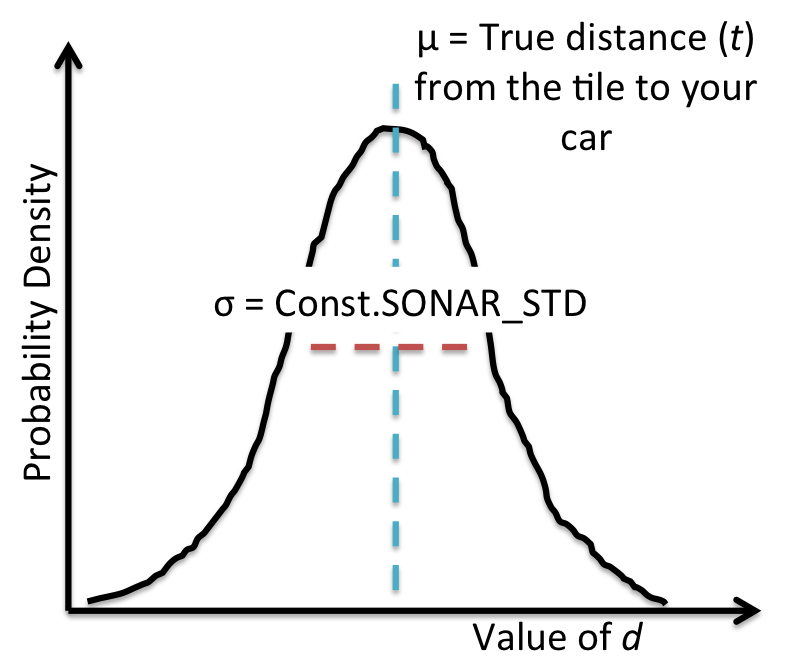
\includegraphics[width=0.5\textwidth]{media/pdf.png}
\end{center}

Your job is to implement a car tracker that (approximately) computes the
posterior distribution $\mathbb P(C_t \mid D_1 = d_1, \dots, D_t = d_t)$ (your
beliefs of where the other car is) and update it for each $t = 1, 2, \dots$.  We
will take care of using this information to actually drive the car (i.e., set
$a_t$ to avoid a collision with $c_t$), so you don't have to worry about that
part.

To simplify things, discretize the world into {\bf tiles} represented by
|(row, col)| pairs, where |0 <= row < numRows| and |0 <= col < numCols|. For
each tile, there is a stored probability representing the belief that there's a car on
that tile. The values can be accessed by: |self.belief.getProb(row, col)|. To
convert from a tile to a location, use |util.rowToY(row)| and
|util.colToX(col)|.

Here's an overview of the assignment components:
  
\begin{itemize}
  \item In Problems 1 and 2 (code), you will implement |ExactInference|, which
  computes a full probability distribution of another car's location over tiles
  |(row, col)|.
  \item In Problem 3 (code), you will implement |ParticleFilter|, which works
  with particle-based representation of this same distribution.
  \item Problem 4 (written) gives you a chance to extend your probability analyses
  to a slightly more realistic scenario where there are multiple other cars and
  you can't automatically distinguish between them.
\end{itemize}
\clearpage

{\bf A few important notes before you get started: }  

\begin{itemize}
\item Past experience suggests that this will be one of the most conceptually
  challenging assignments for many students.  Please start early!
\item You should watch the lectures on Bayesian
networks and HMMs before getting started, and keep the slides handy for
reference while you're working.
\item The code portions of this assignment are short and straightforward -- no
more than about 30 lines in total -- but only if your understanding of the
probability concepts is clear!  (If not, see the previous point.)
\item As a notational reminder: we use the lowercase expressions $p(x)$ or
$p(x\vert y)$ for local conditional probability distributions, which are defined by
the Bayesian network.  We use the uppercase expressions $\mathbb P(X = x)$ or
$\mathbb P(X = x \vert Y = y)$ for joint and posterior probability distributions,
which are not pre-defined in the Bayesian network but can be computed by
probabilistic inference.

Please review the lecture slides for more details.
\end{itemize}

